% =====================================================================
%  Post-Quantum Security of Merkle-Based Transparent Proof Systems
%  COMPLETE PAPER -- single self-contained source.
%
%  Chapters 2-3 reproduce the author's text (from STARK_draft_v2.docx)
%  with the f128 field corrections applied; Chapter 4 (Results) is the
%  measured campaign, with pgfplots figures generated from the data.
%  Figures 1-11 are the author's diagrams (figures/g_*.pdf, converted
%  from the supplied SVGs); Fig. 7 and 12-15 are generated here.
%
%  Compile: pdflatex paper_full.tex  (x2, for refs). Standard CTAN
%  packages only; no shell-escape.
% =====================================================================
\documentclass[11pt]{article}

\usepackage[utf8]{inputenc}
\usepackage[T1]{fontenc}
\usepackage[margin=2.5cm]{geometry}
\usepackage{graphicx}
\usepackage{float}
\usepackage{amsmath}
\usepackage{amssymb}
\usepackage{booktabs}
\usepackage{siunitx}
\usepackage{caption}
\usepackage{pgfplots}
\usepackage{filecontents}
\pgfplotsset{compat=1.18}
\usepgfplotslibrary{groupplots}
\emergencystretch=3em
\usepackage[hidelinks]{hyperref}

\sisetup{group-separator={,}, group-minimum-digits=4}
\graphicspath{{figures/}}

% Include a supplied figure if present, else a labelled placeholder box.
\newcommand{\paperfig}[4]{% #1=name-without-ext (in figures/)  #2=width  #3=caption  #4=label
  \begin{figure}[htbp]\centering
  \IfFileExists{figures/#1.pdf}{\includegraphics[width=#2]{#1}}%
    {\fbox{\parbox[c][2.6cm][c]{#2}{\centering\ttfamily [missing figure: figures/#1.pdf]}}}%
  \caption{#3}\label{#4}\end{figure}}

% Sections are numbered from 1 (Introduction).

% ---------------------------------------------------------------------
%  Measured data embedded for the Results figures (medians of 7 runs).
%  Values verified against the measured dataset.
% ---------------------------------------------------------------------
\begin{filecontents*}[overwrite]{scaling.dat}
n        TC        TP        TPep       TPem      ratio  proofKiB  verify  sec
1024     0.069     0.278     0.009      0.012     4.03   54.56     0.610   111
4096     0.290     1.922     0.347      0.501     6.63   68.81     1.305   111
16384    1.100     7.770     0.046      0.030     7.06   83.54     1.509   111
65536    5.481     33.617    2.077      0.033     6.13   99.33     1.729   111
262144   30.675    146.159   3.675      6.561     4.76   118.83    2.006   111
1048576  125.747   740.649   1955.824   17.813    5.89   138.12    5.850   111
\end{filecontents*}
\begin{filecontents*}[overwrite]{queries.dat}
q    sec   proofKiB   TP       verify
16   47    54.32      34.005   1.222
24   71    77.81      33.781   1.324
32   111   99.33      33.745   2.058
48   127   142.25     34.466   2.611
64   127   183.50     33.685   3.310
\end{filecontents*}
\begin{filecontents*}[overwrite]{digest.dat}
lambda  sec   proofKiB
192     96    80.38
256     111   99.33
\end{filecontents*}
\begin{filecontents*}[overwrite]{grinding.dat}
g    sec   TP        proofKiB
0    95    33.477    98.89
8    103   33.621    100.08
16   111   33.391    99.33
24   119   33.457    99.96
32   127   193.723   100.43
\end{filecontents*}
\begin{filecontents*}[overwrite]{blowup.dat}
b    sec   TP       proofKiB
4    63    20.556   91.29
8    111   33.859   99.33
16   127   61.619   106.89
\end{filecontents*}

\title{\vspace{-1.5em}Post-Quantum Security of Merkle-Based\\Transparent Proof Systems%
\thanks{Source code for the measurement campaign is available at
\url{https://github.com/carlobarbieri5/stark-sperimentazione}.}}
\author{}
\date{}

\begin{document}
\maketitle
\vspace{-2em}

% =====================================================================
\section{Introduction}
\label{sec:intro}

Imagine a receipt thousands of lines long. Out of habit one scans the totals, hoping to catch the
familiar slips: a quantity mismeasured, the wrong item rung up, an arithmetic error buried somewhere in
the column. Re-adding the whole bill by hand, however, is a demanding task, and with limited time or resources it may not be feasible. What one would want instead is a way to be convinced, with something
close to algebraic certainty, that the final figure is right \emph{without} re-checking the receipt line
by line. This dissertation asks whether such verification is possible, and at what price.

Modern cryptography answers yes. A proof system lets a prover convince a verifier that a statement is
true while the verifier does far less work than the computation itself would take; succinct proofs of
this kind already settle batches of blockchain transactions that no single participant could afford to
replay. Most of the efficient systems in use, however, buy their succinctness with a number-theoretic
assumption and a one-time trusted setup. Both are fragile. The assumption is of the kind that
Shor's algorithm dismantles once a large quantum computer exists, and the recent standardisation of
post-quantum cryptography [5] shows that this threat is now treated as real rather than hypothetical.

Transparent STARKs(Scalable Transparent Argument of Knowledge) take a different route. They rest on nothing but a collision-resistant hash function,
so they need no trusted setup and remain standing against a quantum adversary [1]. That robustness is
not free: the proofs are larger and the prover works harder, and exactly how much larger and harder is a
question better answered by measurement than by asymptotics. Yet the empirical cost of these systems
(how prover time, proof size and security move as the parameters a practitioner controls are turned)
is rarely laid out in one place.

This work sets out to fill that gap. It builds a measurement harness around a mature STARK prover and
runs a controlled campaign over a fixed workload, sweeping the proof parameters one at a time and
recording what each costs in prover time, verifier time, proof size and conjectured security. Throughout,
the security figures are Winterfell's \emph{conjectured} estimates, not formal proofs
(Section~\ref{sec:twoterms}). The aim is not a new protocol but an honest map: what transparency and
post-quantum security actually cost, and how the available parameters trade against one another.

The dissertation proceeds as follows. Section~\ref{sec:background} places STARKs among succinct proof
systems and explains why only the hash-based family survives a quantum adversary. Section~\ref{sec:method}
develops just enough of the protocol (arithmetization, commitment, low-degree testing and the two
roles of the hash) to make the measurements readable. Section~\ref{sec:results} reports the campaign;
Section~\ref{sec:discussion} interprets the cost trade and states the limits of the study; and
Section~\ref{sec:conclusions} summarises the findings and the work they leave open.

% =====================================================================
\section{Background}
\label{sec:background}

\subsection{Computational integrity and the limits of na\"ive verification}

This dissertation addresses \emph{computational integrity}: when one party runs a computation and
reports a result, how can others be sure the output is the real one and not a convenient lie?~[1] The
obvious check (rerun and compare, as a new node re-validates a blockchain) does not scale, and
fails outright when the data is confidential (medical or forensic records) and cannot be revealed for
re-execution.~[1] The usual fallback, a trusted human auditor, is a single point of failure that can be
hacked, bribed, or coerced. What we want instead is a proof system whose verification time and
communication grow only with the logarithm of the work and the size of a short commitment to the data,
not with the data itself.~[1]

Succinct proof systems are exactly that: automated protocols that replace the auditor, letting one become
convinced a computation was done correctly while doing far less work than re-running it: ``verify,
don't trust''.~[1][2] Some are also \emph{zero-knowledge}, additionally hiding the sensitive inputs: the
motivating example here is the DNA-profile-match problem, where a police force proves that a candidate's
profile is \emph{not} in a forensic database without revealing either the profile or the database.
Zero-knowledge is an extra property layered on succinctness, though: the configuration measured in this
work provides the integrity guarantee but is \emph{not} zero-knowledge (Section~\ref{sec:setup}). The
same idea reshaped blockchains, whose throughput was historically bounded by every node re-running every
transaction. A succinct proof removes that bound: one untrusted prover executes a large batch and emits
a short proof that every node checks in time logarithmic in the work, the architecture of STARK-based
validity rollups, which realizes the field's founding image:

\begin{quote}
``\,\ldots a single reliable PC can monitor the operation of a herd of supercomputers with powerful
but unreliable software and untested hardware\,\ldots''\\[2pt]
\hspace*{1em}--- Babai, Fortnow, Levin \& Szegedy, 1991~[6]
\end{quote}

In a blockchain that reliable PC is the validator network and the supercomputers are the prover: the
chain becomes the verifier. The rest of this chapter places STARKs in this landscape, explains why they
are post-quantum, and describes the cost of that security.~[1]

\subsection{Proof systems and their cryptographic assumptions}

Before any cryptography, it helps to see the object these systems manipulate. A statement about a long
computation (``from state $x$, after a million transactions of program $P$, the machine reached
$y$'') can be rewritten as a large puzzle of purely \emph{local} constraints, like a Sudoku grid
where each cell is constrained only by its row, column, and box. If every local check passes, the whole
grid is globally correct (Figure~\ref{fig:sudoku}). An honest computation satisfies them all; any cheat
violates a large fraction, so a verifier who samples one random constraint catches the lie with high
probability. This is the move from a probabilistically checkable proof (PCP) to a STARK.

\begin{figure}[H]\centering
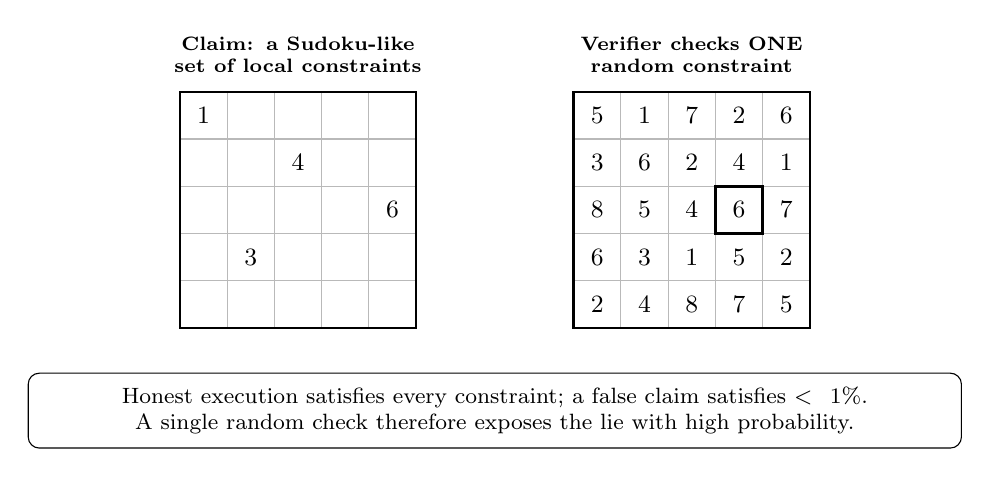
\begin{tikzpicture}[font=\small]
% left grid: the claim (sparse)
\draw[step=0.6cm, gray!55] (0,0) grid (3,3);
\draw[thick] (0,0) rectangle (3,3);
\node[font=\scriptsize\bfseries, align=center, text width=3.4cm, anchor=south] at (1.5,3.12) {Claim: a Sudoku-like set of local constraints};
\node at (0.3,2.7) {1};  \node at (1.5,2.1) {4};  \node at (2.7,1.5) {6};  \node at (0.9,0.9) {3};
% right grid: verifier checks one random constraint
\begin{scope}[xshift=5cm]
\draw[step=0.6cm, gray!55] (0,0) grid (3,3);
\draw[thick] (0,0) rectangle (3,3);
\node[font=\scriptsize\bfseries, align=center, text width=3.4cm, anchor=south] at (1.5,3.12) {Verifier checks ONE random constraint};
\foreach \c/\n in {0/5,1/1,2/7,3/2,4/6} {\node at ({0.3+0.6*\c},2.7) {\n};}
\foreach \c/\n in {0/3,1/6,2/2,3/4,4/1} {\node at ({0.3+0.6*\c},2.1) {\n};}
\foreach \c/\n in {0/8,1/5,2/4,3/6,4/7} {\node at ({0.3+0.6*\c},1.5) {\n};}
\foreach \c/\n in {0/6,1/3,2/1,3/5,4/2} {\node at ({0.3+0.6*\c},0.9) {\n};}
\foreach \c/\n in {0/2,1/4,2/8,3/7,4/5} {\node at ({0.3+0.6*\c},0.3) {\n};}
\draw[very thick] (1.8,1.2) rectangle (2.4,1.8);
\end{scope}
\node[draw, rounded corners, align=center, font=\footnotesize, text width=11.5cm, inner sep=5pt]
  at (4,-1.05) {Honest execution satisfies every constraint; a false claim satisfies $<1\%$.\\
  A single random check therefore exposes the lie with high probability.};
\end{tikzpicture}
\caption{The PCP/STARK intuition. A computation is reduced to a grid of purely local constraints, like a
Sudoku: an honest execution satisfies them all, a false claim violates a large fraction, so checking
one random constraint already exposes the lie with high probability. This is an idealization: a real
proof first encodes the computation (a low-degree extension), so that any cheat disagrees on a large
fraction of points, and only then amplifies soundness over many independent queries (Section~2.4); a
single check on a raw transition would not suffice.}
\label{fig:sudoku}
\end{figure}

Figure~\ref{fig:sudoku} captures only the per-step picture, a single two-dimensional grid of local
constraints, which is the PCP idea. A STARK certifies a computation that runs for many steps, so the same
kind of local check is imposed not once but at \emph{every} step of the execution trace, between each pair
of adjacent rows. The honest object is therefore better imagined as a \emph{stack} of such grids, one
layer per iteration, with a depth equal to the trace length (Figure~\ref{fig:starkstack}). Soundness comes
from sampling random points across this whole stack rather than a single layer, and the encoding of the
trace into low-degree polynomials (Section~\ref{sec:method}) is what makes a handful of such samples
decisive.

\begin{figure}[H]\centering
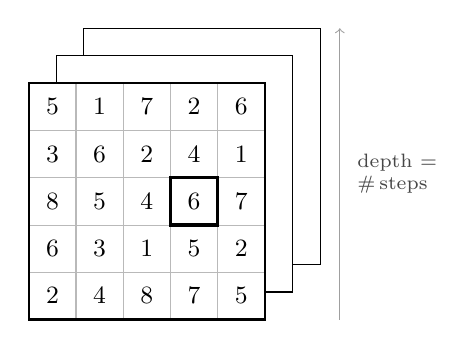
\begin{tikzpicture}[font=\small]
% layers behind (further iterations of the trace): only the border, peeking out top-right
\foreach \o in {0.7, 0.35} {
  \fill[white] (\o,\o) rectangle ({\o+3},{\o+3});
  \draw[thin] (\o,\o) rectangle ({\o+3},{\o+3});
}
% front layer (one step of the trace), fully visible -- reuses the right grid of Figure 1
\fill[white] (0,0) rectangle (3,3);
\draw[step=0.6cm, gray!55] (0,0) grid (3,3);
\draw[thick] (0,0) rectangle (3,3);
\foreach \c/\n in {0/5,1/1,2/7,3/2,4/6} {\node at ({0.3+0.6*\c},2.7) {\n};}
\foreach \c/\n in {0/3,1/6,2/2,3/4,4/1} {\node at ({0.3+0.6*\c},2.1) {\n};}
\foreach \c/\n in {0/8,1/5,2/4,3/6,4/7} {\node at ({0.3+0.6*\c},1.5) {\n};}
\foreach \c/\n in {0/6,1/3,2/1,3/5,4/2} {\node at ({0.3+0.6*\c},0.9) {\n};}
\foreach \c/\n in {0/2,1/4,2/8,3/7,4/5} {\node at ({0.3+0.6*\c},0.3) {\n};}
\draw[very thick] (1.8,1.2) rectangle (2.4,1.8);
% depth = number of iterations
\draw[->, gray!75] (3.95,0) -- (3.95,3.7);
\node[font=\scriptsize, anchor=west, align=left, text=gray!55!black] at (4.05,1.85) {depth $=$\\\#\,steps};
\end{tikzpicture}
\caption{From PCP to STARK. A single grid (Figure~\ref{fig:sudoku}) is one step's worth of constraints; a
real proof stacks one such layer per step of the execution trace, so the constraint system gains a
\emph{depth} equal to the number of iterations. The verifier's random checks probe through all the layers,
not one; the two outlined sheets behind stand for the remaining steps.}
\label{fig:starkstack}
\end{figure}

\subsection{Post-quantum security}

Nearly all succinct proof systems begin with the same move, \emph{arithmetization}: the computation is
reduced to claims about low-degree polynomials over a finite field (``low degree'' meaning far below the
field size). What distinguishes them is not this skeleton but three downstream choices: the field,
the mechanism that enforces low-degreeness, and the cryptographic assumption on which soundness rests
(Figure~\ref{fig:assumptions}).~[2]

\begin{figure}[H]\centering
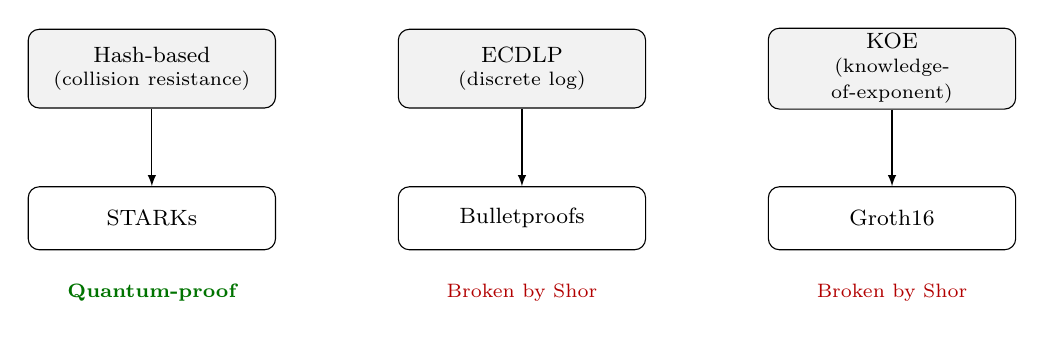
\begin{tikzpicture}[font=\footnotesize, >=latex,
  fam/.style={draw, rounded corners, align=center, text width=3cm, minimum height=1cm, fill=black!5, inner sep=2pt},
  sys/.style={draw, rounded corners, align=center, text width=3cm, minimum height=0.8cm, inner sep=2pt}]
\node[fam] (hash) at (0,1.9)   {Hash-based\\[-1pt]{\scriptsize(collision resistance)}};
\node[fam] (dlp)  at (4.7,1.9) {ECDLP\\[-1pt]{\scriptsize(discrete log)}};
\node[fam] (koe)  at (9.4,1.9) {KOE\\[-1pt]{\scriptsize(knowledge-of-exponent)}};
\node[sys] (stark) at (0,0)   {STARKs};
\node[sys] (bp)    at (4.7,0) {Bulletproofs};
\node[sys] (groth) at (9.4,0) {Groth16};
\draw[->] (hash) -- (stark);
\draw[->] (dlp)  -- (bp);
\draw[->] (koe)  -- (groth);
\node[font=\scriptsize\bfseries, text=green!45!black] at (0,-0.95)   {Quantum-proof};
\node[font=\scriptsize, text=red!70!black]            at (4.7,-0.95) {Broken by Shor};
\node[font=\scriptsize, text=red!70!black]            at (9.4,-0.95) {Broken by Shor};
\end{tikzpicture}
\caption{The three families of proof systems, sorted by cryptographic assumption. Only the hash-based
family is plausibly quantum-resistant; Shor's algorithm breaks the number-theoretic families.}
\label{fig:assumptions}
\end{figure}

Table~\ref{tab:t1} compares the main universal zero-knowledge systems on the properties that matter
here.~[1] Only one construction combines a scalable prover, a scalable verifier, transparency, and
post-quantum security: the STARK.~[1]

\begin{table}[htbp]\centering\footnotesize
\caption{Universal (NP-complete) realized zero-knowledge systems compared on the four properties
relevant to this work; reconstructed from Ben-Sasson et al.~[1, Fig.~2]. hPKC = homomorphic-public-key
SNARKs (e.g.\ Groth16, KZG-based PLONK); DLP = discrete-logarithm arguments with no trusted setup
(e.g.\ Bulletproofs); MPC = MPC-in-the-head arguments (e.g.\ Ligero, ZKBoo); ZK-STARK = the hash-and-FRI
construction of~[1].}
\label{tab:t1}
\begin{tabular}{l c c c c}
\toprule
Approach & Prover scalable & Verifier scalable & Transparent & Post-quantum \\
         & (quasilinear)   & (polylog)         &             &              \\
\midrule
hPKC     & Yes & Only if repeated & No  & No  \\
DLP      & Yes & No               & Yes & No  \\
MPC      & Yes & No               & Yes & Yes \\
ZK-STARK & Yes & Yes              & Yes & Yes \\
\bottomrule
\end{tabular}
\end{table}

``Post-quantum'' means relying only on assumptions not known to fall to a large-scale quantum computer.
Shor's algorithm solves factoring and the discrete logarithm efficiently, breaking RSA and
elliptic-curve cryptography and with them the second and third families above.~[1][2] The first family
survives: no quantum algorithm is known to break collision-resistant hashing, which is exactly why
STARKs are post-quantum candidates.~[1][2]

Surviving is not the same as being unaffected, and it helps to be precise about \emph{which} property
erodes. Two different attacks matter, and they bite differently. Against \emph{preimage} resistance,
Grover's algorithm cuts a brute-force search from $2^{n}$ to $2^{n/2}$, so an $n$-bit hash keeps only
$n/2$ bits against a quantum attacker~[7]. What a Merkle commitment actually relies on, though, is
\emph{collision} resistance (Section~3.4): this is already the weaker of the two even classically
(the birthday bound makes a collision cost only $2^{n/2}$, not $2^{n}$), and Brassard--H\o yer--Tapp
lowers it further to $2^{n/3}$ on a quantum machine, an attack that needs a large quantum memory of
doubtful feasibility~[8]. The practical security is therefore taken at the classical birthday level
$\lambda/2$: a $192$-bit digest caps near $96$ bits ($=192/2$), exactly as Section~\ref{sec:twoterms}
measures. This is the convention behind Winterfell's reported figures: the hash term is a \emph{classical}
birthday estimate, not a quantum-reduced bound, so the post-quantum claim of this thesis rests on the
\emph{assumption} surviving Shor, not on a quantum-adjusted bit count. The defence is the same and cheap
in every case (lengthen the hash output) and is one of the parameters the experiments vary.

Crucially, this security follows from the \emph{choice of assumption}, not from a patch added later: a
system that commits with hash functions and tests low-degreeness information-theoretically is
quantum-resistant for free, whereas an elliptic-curve commitment cannot be.~[1][2] This puts STARKs in
the same family as the post-quantum signatures standards bodies now endorse: in August 2024 NIST
finalized FIPS 203/204/205, the last of which (a stateless hash-based signature) rests, like a
Merkle-based STARK, on nothing but a hash function.~[5][1]

\subsection{The price of transparency and post-quantum security}

The mechanism that enforces low-degreeness is where the assumption enters, and the three families use
three commitment schemes with very different costs (Table~\ref{tab:t2}): a STARK uses FRI (hash-based),
the discrete-log family uses inner-product arguments, and the pairing family uses KZG.~[2]

\begin{table}[htbp]\centering\footnotesize
\caption{The three commitment schemes used to enforce low-degreeness, compared on cost and assumption;
after Ben-Sasson~[2]. IPA = inner-product argument; KZG = Kate--Zaverucha--Goldberg.}
\label{tab:t2}
\begin{tabular}{l l l l}
\toprule
Property & FRI (STARK) & Inner-product argument & KZG \\
\midrule
Verifier     & Succinct                & Linear-time           & Succinct (short) \\
Setup        & Transparent, succinct   & Transparent           & Trusted, linear size/time \\
Proof size   & Large (tens of KB)      & Short (KBs)           & Very short ($<1$ KB) \\
Post-quantum & Yes                     & No                    & No \\
Assumption   & Collision-resistant hash& Discrete-log hardness & Knowledge-of-exponent \\
\bottomrule
\end{tabular}
\end{table}

The bargain is explicit: FRI is the only one of the three that is at once transparent, post-quantum, and
usable over any finite field, but it pays in proof size: tens of kilobytes against a sub-kilobyte KZG
proof, about three orders of magnitude (roughly $1000\times$) larger than a pairing-based SNARK.~[1][2]
Transparency and quantum resistance are bought with bytes.

Most of those bytes are the Merkle authentication paths that accompany the verifier's queries. To first
order the communication cost is the number of queries times the field-element size, plus the number of
authentication-path nodes times the hash length $\lambda$:~[1]
\begin{equation}
  |\pi| \;\approx\; q_{\mathrm{total}}\cdot \log_2|\mathbb{F}| \;+\; \mathrm{AP}_{\mathrm{total}}\cdot \lambda .
  \label{eq:commcost}
\end{equation}
Each symbol is one measurable quantity of a proof:

\begin{table}[htbp]\centering\footnotesize
\begin{tabular}{l p{0.78\linewidth}}
\toprule
Term & Meaning \\
\midrule
$q_{\mathrm{total}}$ & The total number of queries the verifier makes into the committed data. More
queries raise soundness (each is an independent chance to catch a cheating prover) but add data
to send. \\[2pt]
$\log_2|\mathbb{F}|$ & The number of bits needed to write one field element, i.e.\ the size of a single
answer returned at a queried point. For the $128$-bit prime field \texttt{f128} used here (modulus
$2^{128}-45\cdot2^{40}+1$) this is \textbf{$128$ bits}. \\[2pt]
$\mathrm{AP}_{\mathrm{total}}$ & The total number of Merkle authentication-path nodes sent across all
queries. Each queried leaf must carry the sibling hashes on its path to the root so the verifier can
recompute the root; this is the dominant term. \\[2pt]
$\lambda$ & The hash output length in bits, the size of one tree node. Lengthening $\lambda$ is the
defence against Grover's attack on the hash, and it directly inflates the authentication-path term. \\
\bottomrule
\end{tabular}
\end{table}

The first product is the cost of the answers; the second, of proving they were the committed ones. The two
are linked: each query carries one authentication path, so $\mathrm{AP}_{\mathrm{total}}\approx
q_{\mathrm{total}}\times$ the Merkle-tree depth $\approx q_{\mathrm{total}}\log_2(\text{domain size})$, and
the second term (of order $q_{\mathrm{total}}\,\lambda\log_2(\text{domain})$) is the one that
dominates. This first-order model is the hinge of the experiments: every defensive increase (more
queries, or a longer hash to restore the bits Grover removes) enlarges one of these terms, and so the
proof. Concretely, the queries sweep (Section~\ref{sec:twoterms}) varies $q_{\mathrm{total}}$, the digest
sweep varies $\lambda$, and blowup and FRI folding move $\mathrm{AP}_{\mathrm{total}}$; none of these is
read off directly, only \emph{indirectly} through the proof size Winterfell reports. The Results chapter
measures that growth; here we only locate its source.

% =====================================================================
\section{Methodology}
\label{sec:method}

This chapter explains just enough of the STARK protocol to make the measurements readable: how a
computation becomes a set of polynomial constraints (arithmetization), how those constraints turn into a
short proof (commitment, querying, and low-degree testing), and the two places where the hash function
enters: the Merkle commitment (which needs collision resistance) and the Fiat--Shamir transform (which
needs random-oracle behaviour), and with them the post-quantum question. A small worked example shows the template in
isolation. What this chapter does \emph{not} do is reprove the theory: the formal proofs that the
protocol is sound, and the engineering optimizations that make a real implementation fast, are left to
the works it builds on~[1][2]. The aim here is the working understanding needed to read the
measurements, not complete rigour.

\subsection{Arithmetization: from computation to polynomial constraints}

Arithmetization turns a claim about a computation into a claim about polynomials over a finite
field.~[1] The claim has the canonical form ``$\alpha$ is the result of running program $C$ for $T$
steps on public input $x$'' (the DNA-match statement is a special case). It proceeds in stages. First,
the execution of $C$ is recorded as an \emph{execution trace}: a table whose rows are the successive
states and whose columns are the tracked registers; a computation of $n$ data elements at $c$ cycles
each gives $c\cdot n$ rows and a fixed width $w$ (Table~\ref{tab:trace}).~[1]

\begin{table}[htbp]\centering\footnotesize
\caption{An execution trace: one row per step, one column per register. The example follows the
recurrence $x \mapsto x^{3}+42$ starting at $3$, over the $128$-bit prime field \texttt{f128}
(Section~\ref{sec:field}); the final state is reduced modulo $p$.}
\label{tab:trace}
\begin{tabular}{c c}
\toprule
Step & State \\
\midrule
0          & 3 \\
1          & 69 \\
2          & 328551 \\
3          & $\vdots$ \\
$c\cdot n$ & \num{247770943907079986105389697876176586605} \\
\bottomrule
\end{tabular}
\end{table}

Second, the rules a legal step must obey become an \emph{algebraic intermediate representation} (AIR):
low-degree polynomials $P_1,\ldots,P_s$ over the current and next state. A pair $(\vec{s},\vec{s}\,')$ is
a valid transition exactly when all of them vanish on it,~[1]
\begin{equation}
  P_1(\vec{s},\vec{s}\,') = \cdots = P_s(\vec{s},\vec{s}\,') = 0,
\end{equation}
so that the AIR captures the entire step relation as a system of polynomial equations.

An AIR has three ingredients~[3]. \emph{Public inputs}: values prover and verifier agree on, typically
the start $x$ and asserted result $y$. \emph{Transition constraints}: the polynomials above, zero on
every legal step and non-zero on any illegal one; their highest degree is the constraint degree $d$ that
drives cost. \emph{Boundary assertions}: pin specific trace cells to fixed values (usually the first row
to the input and the last to the output). A trace satisfies the AIR when every transition constraint
vanishes on adjacent rows and every boundary assertion holds.

For the running example $x\mapsto x^{3}+42$ of Table~\ref{tab:trace}, the three become concrete. The
public inputs are the start $x=3$ and the claimed result $y$. The single transition constraint is
$P(s,s')=s'-(s^{3}+42)$, which is zero exactly when the next state is the cube-plus-$42$ of the current
one, and whose degree is the constraint degree $d=3$. The boundary assertions pin the first cell to $3$
and the last to $y$. The trace is accepted precisely when $P$ vanishes between every pair of adjacent
rows and both boundary cells match, e.g.\ the step $3\mapsto 69$ satisfies $69-(3^{3}+42)=0$.

Third, each trace column is interpolated into a polynomial over an evaluation domain; applying the AIR
to these trace polynomials yields a constraint polynomial that vanishes on the step-points exactly when
the computation is honest.~[2]

Four AIR parameters drive all downstream cost (width $w$, cycles $c$, constraint degree $d$, and the
number of constraints $s$), so minimizing them is the craft of this stage.~[1] Since the benchmark's
expensive part is repeated hashing, the choice of hash dominates these parameters; Table~\ref{tab:t3}
gives them for three standard primitives and the benchmark.~[1] The gap between rows is what the
experiments probe when they vary the hash backend.

\begin{table}[htbp]\centering\footnotesize
\caption{Principal AIR parameters for three cryptographic primitives and the benchmark program, per
data element; reconstructed from Ben-Sasson et al.~[1, Fig.~4]. The final column is the total number of
multiplication gates of the equivalent arithmetic circuit.}
\label{tab:t3}
\begin{tabular}{l r r r r}
\toprule
Primitive (core repeated operation) & State width $w$ & Cycles $c$ & Constraint degree $d$ & Mult.\ gates (per element) \\
\midrule
SHA-2                       & 56 & 3762 & 11 & \num{2708640} ($\approx 2^{21.3}$) \\
AES-128 + Davies--Meyer     & 62 & 48   & 8  & \num{23328} ($\approx 2^{14.5}$) \\
Rijndael-160 + Davies--Meyer& 68 & 58   & 8  & \num{51678} ($\approx 2^{15.7}$) \\
DNA-profile-match (benchmark)& 81 & 62  & 8  & \num{90954} ($\approx 2^{16.4}$) \\
\bottomrule
\end{tabular}
\end{table}

Figure~\ref{fig:multgates} plots that last column on a logarithmic axis. The gap is stark: SHA-2 needs
roughly thirty to a hundred times more multiplications than the arithmetization-friendly alternatives,
which is why the hash choice dominates a STARK's cost and is the main variable of the experiments.

\begin{figure}[htbp]\centering
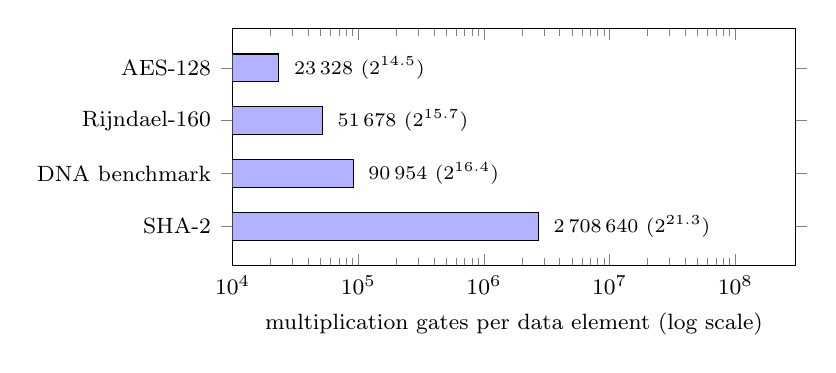
\begin{tikzpicture}
\begin{axis}[
  xbar, xmode=log, width=0.72\linewidth, height=4.6cm,
  xlabel={multiplication gates per data element (log scale)},
  xmin=10000, xmax=300000000,
  xtick={1e4,1e5,1e6,1e7,1e8},
  ytick={1,2,3,4}, yticklabels={SHA-2, DNA benchmark, Rijndael-160, AES-128},
  tick label style={font=\footnotesize}, label style={font=\footnotesize},
  point meta=explicit symbolic,
  nodes near coords, nodes near coords style={anchor=west, xshift=2pt, font=\scriptsize},
  enlarge y limits=0.25, bar width=10pt,
]
\addplot[fill=blue!30] coordinates {(2708640,1)[\num{2708640} ($2^{21.3}$)] (90954,2)[\num{90954} ($2^{16.4}$)] (51678,3)[\num{51678} ($2^{15.7}$)] (23328,4)[\num{23328} ($2^{14.5}$)]};
\end{axis}
\end{tikzpicture}
\caption{Multiplication gates per data element for each primitive (logarithmic axis). SHA-2 costs one
to two orders of magnitude more than the arithmetization-friendly alternatives, the reason the hash
choice dominates a STARK's cost. Data from Table~\ref{tab:t3}.}
\label{fig:multgates}
\end{figure}

One implementation detail matters for the later numbers.\label{sec:field} The system works over the
$128$-bit prime field \texttt{f128}, with modulus
\begin{equation}
  p \;=\; 2^{128} - 45\cdot 2^{40} + 1 \;=\; \text{\num{340282366920938463444927863358409264577}} .
  \label{eq:field}
\end{equation}
This prime is chosen for two reasons. First, $p-1$ is divisible by $2^{40}$, so the field contains
multiplicative subgroups whose size is a power of two, up to $2^{40}$; the FFT and FRI both proceed by
repeatedly halving a domain of power-of-two size, and need exactly such subgroups to exist. Second, $128$
bits fit in two machine words, keeping arithmetic fast on $64$-bit hardware. The trade-off is that the
field holds only about $2^{128}$ values, so no security level drawn from it can exceed $\approx\!128$
bits: near that ceiling the field size itself becomes the limit (the \emph{binding cap}), and going
higher needs a larger \emph{extension} field, the quadratic extension the Results chapter measures.~[3]
The same choice also fixes the scope of the hash comparison in this work: an algebraic hash defined only
over the $64$-bit Goldilocks field cannot operate over \texttt{f128}, so the arithmetization-friendly
Rescue option is field-incompatible here and the comparison is limited to the general-purpose Blake3 and
SHA3 families (the failed attempt is detailed in Section~\ref{sec:nothash}).

\subsection{An idealized commitment and its core check}

To show the template with only the algebra (the cryptography returns in Section~3.4), we use an ideal
commitment scheme with a trusted third party, Tom. Bob (prover) knows a polynomial; Alice (verifier)
wants to check a property of it without seeing it in full; Tom is a trusted store. Alice fixes a field
$\mathbb{F}$ and a degree bound $d$; Bob sends $P\in\mathbb{F}[X]$ with $\deg P<d$ to Tom; later Alice
queries any $a\in\mathbb{F}$ and Tom returns $P(a)$ (Figure~\ref{fig:tom}). Since Tom is trusted, the
stored object is guaranteed to be a genuine degree-$<d$ polynomial: no low-degree test is needed, the
job FRI takes over once Tom is removed.

\begin{figure}[htbp]\centering
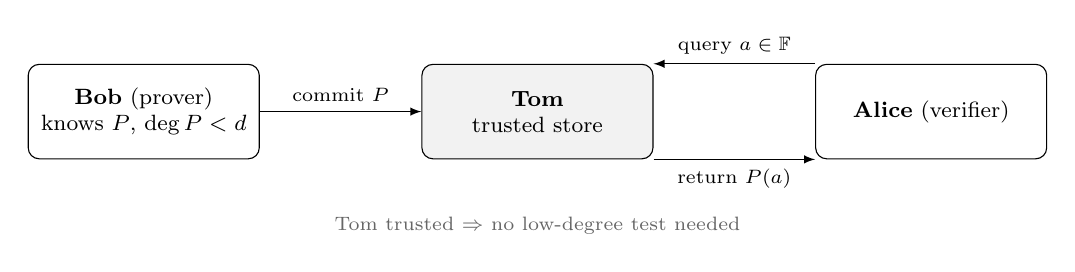
\begin{tikzpicture}[font=\footnotesize, >=latex,
  box/.style={draw, rounded corners, align=center, minimum height=1.2cm, text width=2.7cm}]
\node[box] (bob)   at (0,0)  {\textbf{Bob} (prover)\\knows $P$, $\deg P<d$};
\node[box, fill=black!5] (tom) at (5,0) {\textbf{Tom}\\trusted store};
\node[box] (alice) at (10,0) {\textbf{Alice} (verifier)};
\draw[->] (bob.east) -- node[above, font=\scriptsize]{commit $P$} (tom.west);
\draw[->] (alice.north west) -- node[above, font=\scriptsize]{query $a\in\mathbb{F}$} (tom.north east);
\draw[->] (tom.south east) -- node[below, font=\scriptsize]{return $P(a)$} (alice.south west);
\node[font=\scriptsize, text=black!60, align=center] at (5,-1.45)
  {Tom trusted $\Rightarrow$ no low-degree test needed};
\end{tikzpicture}
\caption{The idealized commitment scheme. Bob sends a bounded-degree polynomial to the trusted store
Tom; Alice later queries Tom at any field point. Because Tom is trusted, no low-degree test is needed:
the job FRI performs once Tom is removed.}
\label{fig:tom}
\end{figure}

Two facts underlie every check. Fix a field $\mathbb{F}$ and a finite $H\subseteq\mathbb{F}$. First,
\emph{vanishing is divisibility}: $P$ vanishes on all of $H$ iff it is divisible by the vanishing
polynomial $Z_H$, i.e.\ $P=Z_H\,Q$ for some quotient $Q$,
\begin{equation}
  P(X) = Z_H(X)\,Q(X).
\end{equation}
When $H$ is a multiplicative group $Z_H$ collapses to a form the verifier evaluates by itself in
logarithmic time:
\begin{equation}
  Z_H(X) = \prod_{h\in H}(X-h) = X^{|H|}-1 .
\end{equation}
Second, \emph{distinct low-degree polynomials rarely agree}: two distinct degree-$<d$ polynomials agree
on at most $d$ points, so over a field much larger than $d$ a single random query separates them,
exposing a false identity, except with probability $\le d/|\mathbb{F}|$.

The pattern is always the same. Bob's claim about $P$ is rewritten as one identity ``(something from
$P$) $=Z_H\cdot Q$'' that holds everywhere iff the claim is true, with $Q$ also committed to Tom. Alice
samples one random $\alpha$, asks for $P(\alpha)$ and $Q(\alpha)$, and accepts iff the identity holds
there. A true claim always passes; a false one fails as a polynomial, so by the few-agreements fact it
survives at only a vanishing fraction of points, and a random $\alpha$ catches it. The next section runs
this on two concrete claims.

\subsection{Two worked examples}

Both examples use the ideal scheme and differ only in the identity tested.

\paragraph{Claim 1: the committed polynomial $P$, of degree below $d$, vanishes on the set $H$.}
\emph{Protocol.} Bob commits to $P$ and to a claimed quotient $Q$ of degree below $d-|H|$. Alice
samples a random point $\alpha \in \mathbb{F}$, queries Tom for $P(\alpha)$ and $Q(\alpha)$, and
accepts if and only if
\begin{equation}
  P(\alpha) = Z_H(\alpha)\,Q(\alpha).
\end{equation}
\emph{Efficiency.} Two queries and $O(\log|H|)$ field operations, on top of the commitment cost:
Alice computes $Z_H(\alpha)$ herself, cheaply, using the multiplicative-group form. \emph{Soundness.}
The error probability is below $d/|\mathbb{F}|$. \emph{Why.} If $P$ vanishes on $H$, divisibility
supplies a $Q$ making the identity hold everywhere, so honest provers pass. If not, $P-Z_HQ$ is a
non-zero degree-$<d$ polynomial with fewer than $d$ roots, so at most $d$ points could fool Alice and a
random $\alpha$ catches the lie except with probability $d/|\mathbb{F}|$.

\begin{figure}[htbp]\centering
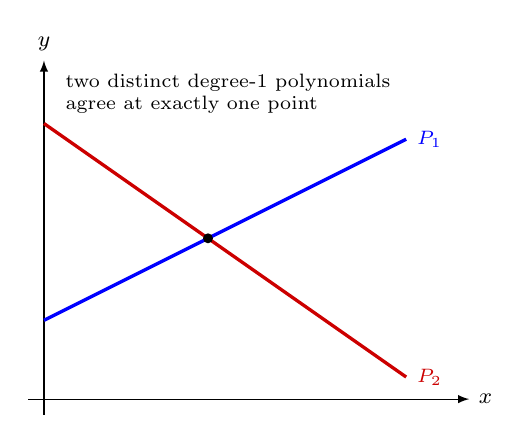
\begin{tikzpicture}[font=\footnotesize, >=latex]
\draw[->] (-0.2,0) -- (5.4,0) node[right] {$x$};
\draw[->] (0,-0.2) -- (0,4.3) node[above] {$y$};
\draw[very thick, blue]         (0,1.0) -- (4.6,3.3) node[right, font=\scriptsize] {$P_1$};
\draw[very thick, red!80!black] (0,3.5) -- (4.6,0.28) node[right, font=\scriptsize] {$P_2$};
\fill (2.083,2.042) circle (1.8pt);
\node[anchor=north west, font=\scriptsize, align=left] at (0.15,4.25)
  {two distinct degree-$1$ polynomials\\agree at exactly one point};
\end{tikzpicture}
\caption{Two distinct lines (degree $1$) meet at most once: the degree-$1$ case of the few-agreements
fact. In general two distinct polynomials of degree below $d$ agree on fewer than $d$ points.}
\label{fig:lines}
\end{figure}

\paragraph{Claim 2: the committed polynomial $P$, of degree below $d$, takes only the values $0$ and
$1$ on $H$}, a ``Boolean'' constraint of the kind that pervades real arithmetizations.
\emph{Protocol.} Only the identity changes. Bob commits to $P$ and to a quotient $Q$, now of degree
below $2d-|H|$; Alice samples $\alpha$, queries $P(\alpha)$ and $Q(\alpha)$, and accepts if and only if
\begin{equation}
  P(\alpha)\bigl(1-P(\alpha)\bigr) = Z_H(\alpha)\,Q(\alpha).
\end{equation}
The product $P(\alpha)(1-P(\alpha))$ vanishes at a point exactly when $P$ is $0$ or $1$ there, so the
identity holds across $H$ exactly when $P$ is Boolean on $H$. \emph{Efficiency.} Again two queries and
$O(\log|H|)$ field operations. \emph{Soundness.} Doubling the degree of the tested polynomial to $2d$
doubles the bound: the error probability is below $2d/|\mathbb{F}|$. \emph{Why it works.} If $P$ is
Boolean on $H$ the product vanishes on $H$ and a valid quotient exists, so honest provers always pass.
If $P$ takes any other value on $H$, then $P(X)(1-P(X))$ does not vanish on $H$, the left-hand side is a
non-zero polynomial of degree $2d$, at most $2d$ points are erroneous, and a random $\alpha$ catches
the violation except with probability $2d/|\mathbb{F}|$.

The lesson generalizes: any property expressible as a single algebraic identity is verified at one
random point, with soundness set by the identity's degree over the field size; a full STARK is many such
reductions composed. What it cannot assume is a trusted Tom: no real party can be relied on to store a
genuine low-degree polynomial. Removing Tom (a real commitment, plus a test that the committed data is
really low-degree and not engineered noise) is exactly what brings in the hash function, and with it the
post-quantum question.

\subsection{Where the hash function enters: two roles, two guarantees}

Making the protocol real means supplying the two things Tom provided: a binding commitment, and the
guarantee that what was committed is genuinely low-degree. The first is where the hash appears. In place
of Tom, the prover evaluates the polynomial over the domain and builds a Merkle tree of those values,
sending only the root (Figure~\ref{fig:merkle}); a query is answered by the leaf plus its authentication
path (the sibling hashes up to the root), and the verifier recomputes the root to confirm the value.
This is a polynomial commitment built from nothing but a hash.~[1][2]

\begin{figure}[htbp]\centering
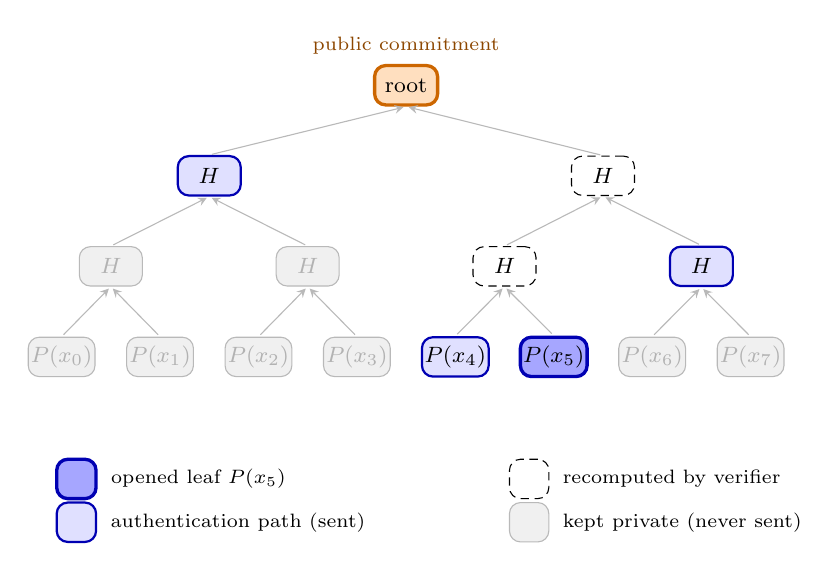
\begin{tikzpicture}[>=stealth, font=\footnotesize,
  cell/.style={draw, rounded corners, minimum width=8mm, minimum height=5mm, inner sep=1pt},
  hidden/.style={cell, draw=gray!55, fill=gray!12, text=gray!60},
  pathn/.style={cell, draw=blue!70!black, fill=blue!12, thick},
  query/.style={cell, draw=blue!70!black, fill=blue!35, very thick},
  recomp/.style={cell, draw=black, densely dashed, fill=white},
  rootn/.style={cell, draw=orange!80!black, fill=orange!25, very thick},
  ed/.style={->, gray!55, shorten >=1pt, shorten <=1pt}]
\def\lx{1.25}
% leaves: the polynomial's evaluations
\node[hidden] (L0) at (0*\lx,0) {$P(x_0)$};
\node[hidden] (L1) at (1*\lx,0) {$P(x_1)$};
\node[hidden] (L2) at (2*\lx,0) {$P(x_2)$};
\node[hidden] (L3) at (3*\lx,0) {$P(x_3)$};
\node[pathn]  (L4) at (4*\lx,0) {$P(x_4)$};
\node[query]  (L5) at (5*\lx,0) {$P(x_5)$};
\node[hidden] (L6) at (6*\lx,0) {$P(x_6)$};
\node[hidden] (L7) at (7*\lx,0) {$P(x_7)$};
% level 1: each node hashes its two children
\node[hidden] (a) at (0.5*\lx,1.15) {$H$};
\node[hidden] (b) at (2.5*\lx,1.15) {$H$};
\node[recomp] (c) at (4.5*\lx,1.15) {$H$};
\node[pathn]  (d) at (6.5*\lx,1.15) {$H$};
% level 2
\node[pathn]  (e) at (1.5*\lx,2.3) {$H$};
\node[recomp] (f) at (5.5*\lx,2.3) {$H$};
% root = commitment
\node[rootn]  (R) at (3.5*\lx,3.45) {root};
\node[anchor=south, font=\scriptsize, text=orange!55!black] at (R.north) {public commitment};
% edges (child -> parent)
\foreach \p/\ch in {a/L0,a/L1,b/L2,b/L3,c/L4,c/L5,d/L6,d/L7,e/a,e/b,f/c,f/d,R/e,R/f}
  \draw[ed] (\ch.north) -- (\p.south);
% legend
\begin{scope}[shift={(0.15*\lx,-1.55)}, font=\scriptsize]
  \node[query,  minimum width=5mm] (g1) at (0,0)        {}; \node[anchor=west] at (g1.east) {\,opened leaf $P(x_5)$};
  \node[pathn,  minimum width=5mm] (g2) at (0,-0.55)    {}; \node[anchor=west] at (g2.east) {\,authentication path (sent)};
  \node[recomp, minimum width=5mm] (g3) at (4.6*\lx,0)  {}; \node[anchor=west] at (g3.east) {\,recomputed by verifier};
  \node[hidden, minimum width=5mm] (g4) at (4.6*\lx,-0.55){}; \node[anchor=west] at (g4.east) {\,kept private (never sent)};
\end{scope}
\end{tikzpicture}
\caption{The Merkle commitment that replaces Tom. The leaves are the polynomial's evaluations; each
internal node hashes its two children; only the root is published (the commitment). A query opens one
leaf, $P(x_5)$, together with its \emph{authentication path}, the sibling hashes on the way up
(blue), from which the verifier recomputes the nodes on that path (dashed) and checks the root. Every
other evaluation and off-path node stays private (grey): the commitment reveals nothing else.}
\label{fig:merkle}
\end{figure}

A binding commitment alone is not enough: a cheating prover could commit to an arbitrary table of values
engineered to satisfy the identity at the few likely query points, while being nothing like a low-degree
polynomial.~[1] The Fast Reed--Solomon IOP of Proximity (FRI) forecloses this, convincing the verifier
that the committed object is \emph{close} to a low-degree polynomial rather than such noise~[1] by
repeatedly folding it in half, halving its degree over a logarithmic number of rounds
(Figure~\ref{fig:fri}).~[2] The work is asymmetric as wanted (linear for the prover, logarithmic for
the verifier), with a soundness error of about $2^{-128}$: the probability that a prover who committed to
something that is \emph{not} a low-degree polynomial still slips past every random check. To picture the
scale, $2^{-128}$ is roughly the chance of guessing one specific $128$-bit key on the first try. This
figure is an idealized target for the FRI low-degree test, and follows from its proximity-gaps bound over
the \texttt{f128} field~[9]; the \emph{conjectured} security actually reported is parameter-dependent
(Section~\ref{sec:twoterms}), $111$ bits at the baseline and rising to the ${\approx}127$-bit field
ceiling. So $2^{-128}$ is the order of magnitude the design aims at, not the baseline figure.

\begin{figure}[htbp]\centering
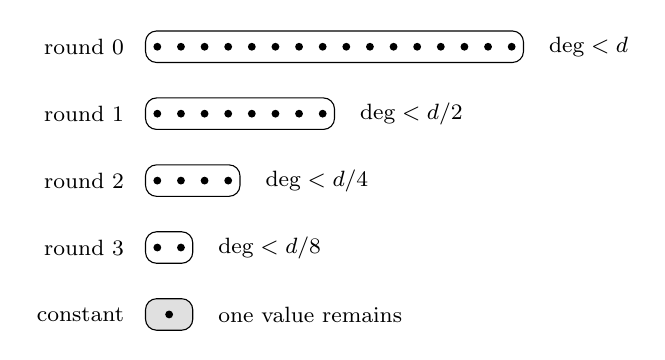
\begin{tikzpicture}[font=\footnotesize, dot/.style={circle, fill=black, inner sep=1pt}]
\foreach \r/\n/\dg/\y in {0/16/{$\deg<d$}/0, 1/8/{$\deg<d/2$}/-0.85, 2/4/{$\deg<d/4$}/-1.7, 3/2/{$\deg<d/8$}/-2.55} {
  \node[anchor=east] at (-0.15,\y) {round \r};
  \pgfmathsetmacro{\w}{\n*0.3}
  \draw[rounded corners] (0,\y-0.2) rectangle (\w,\y+0.2);
  \foreach \i in {1,...,\n} {\node[dot] at ({(\i-0.5)*0.3},\y) {};}
  \node[anchor=west] at (\w+0.2,\y) {\dg};
}
\node[anchor=east] at (-0.15,-3.4) {constant};
\draw[rounded corners, fill=black!12] (0,-3.6) rectangle (0.6,-3.2);
\node[dot] at (0.3,-3.4) {};
\node[anchor=west] at (0.8,-3.4) {one value remains};
\end{tikzpicture}
\caption{FRI folds the committed polynomial roughly in half each round, halving its degree over $\log d$
rounds until a single constant remains (prover work $O(d)$, verifier work $O(\log d)$); the verifier
checks consistency between consecutive layers at random points.}
\label{fig:fri}
\end{figure}

Two features of FRI matter here. Its soundness is information-theoretic: it rests on the geometry of
Reed--Solomon codes and the conjectured proximity-gaps property~[9], not on any computational hardness,
so a quantum computer finds nothing to speed up inside FRI.~[2] And the protocol, interactive so far, is
made non-interactive, where the hash appears a second time.

A non-interactive STARK thus uses a hash in two distinct ways: keeping them apart is the spine of
this dissertation. The first is the Merkle commitment above: it needs \emph{collision resistance}, since
an adversary who finds two values hashing to the same node could open the commitment inconsistently and
break soundness.~[1][3] The second is the Fiat--Shamir transform, which removes interaction by deriving
the query points from a hash of the transcript so far; this needs the hash to act like an unbiased
\emph{random oracle}, so the prover cannot steer the ``random'' challenges.~[1][2]

This split has a formal counterpart: an interactive STARK follows from collision-resistant hashing alone
(Kilian's transformation), while the non-interactive one used in practice needs the stronger
random-oracle assumption (Micali/Valiant).~[1] The interactive route needs the weaker guarantee; the
deployed non-interactive route needs both.

The separation of roles mirrors a separation of information (Table~\ref{tab:t4}): what the verifier needs
for its challenges is public, while the witness stays private, exposed only as point-values at the
queried points.~[2]

\begin{table}[htbp]\centering\footnotesize
\caption{The protocol's information flow: what the verifier may see (public) versus what the prover
keeps (private), revealed only as individual evaluations at the queried points.}
\label{tab:t4}
\begin{tabular}{p{0.45\linewidth} p{0.45\linewidth}}
\toprule
Public & Private \\
\midrule
The AIR, with its transition constraints and boundary assertions & The execution trace \\
The vanishing polynomial $Z_H$            & The trace and constraint polynomials \\
The commitments (Merkle roots)            & The quotient polynomial $Q$ \\
The query points / challenges             & Revealed only as point-values $P(\alpha),Q(\alpha)$ at the queried $\alpha$ \\
\bottomrule
\end{tabular}
\end{table}

The two roles meet two different quantum attacks and two different defences, which the experiments
make concrete. Against the Merkle commitment the threat is Grover's quadratic speedup on collision and
preimage search; the defence is a longer hash output, paid for in proof size through the
authentication-path term of Section~2.4. Against Fiat--Shamir it is subtler: classical arguments do not
automatically survive a quantum adversary querying the hash in superposition (the quantum random-oracle
model), and the difficulty is sharper for many-round protocols like FRI~[10]. The same hash is asked for
two things, attacked two ways, and defended two ways: the separation this dissertation isolates.

The implementation states the separation explicitly: the conjectured security of a proof is the smaller
of two terms: an information-theoretic FRI term (from the queries, code parameters, and a proof-of-work
``grinding'' factor) and the collision resistance of the chosen hash.~[4] The grinding term is itself
subject to Grover and must roughly double its bits against a quantum attacker; the hash term is the one a
longer digest protects.~[4] Varying these terms independently, and measuring the cost of each, is the
task of the Results chapter.

% =====================================================================
\section{Results}
\label{sec:results}

The workload is a Rescue--Prime hash chain of length~$n$ (Rescue--Prime is an
\emph{arithmetization-friendly} hash, built from few field multiplications so that proving it inside a
STARK is cheap), so the cost of each step is dominated by hashing (Section~3.1); the prover proves that the public result is the $n$-fold Rescue image of the
public seed, and we measure what that proof costs. For each configuration the prover and verifier were
timed over seven repetitions after one discarded warm-up, and we report the median with the run-to-run
range as $[\min,\max]$; the native baseline $T_C$ (Section~\ref{sec:scaling}) is instead measured
\emph{once} per configuration, and that single value is reused for the configuration's seven rows. Two points
are worth keeping in mind. First, the security figure is Winterfell's \emph{conjectured} value, not a
proven bound: ``conjectured'' means the library computes it on two standard but unproven assumptions. The
first concerns \emph{FRI}, the low-degree test at the core of the proof: from a handful of random samples
it lets the verifier conclude that the committed data really is a genuine low-degree polynomial, and not
noise engineered to pass the checks; the assumption (its \emph{proximity-gaps} soundness~[9]) is that
this conclusion fails only with the tiny probability claimed. The second is that Fiat--Shamir, the
hashing trick that makes the protocol non-interactive, behaves like an ideal \emph{random oracle}~[10].
Both are widely believed; granting them, the reported security is the smaller of an information-theoretic
(FRI) term and a hash term (Section~\ref{sec:twoterms}). Second, on a single laptop, absolute proving
times carry thermal noise, so read them for their \emph{trends}, not their exact values; the deterministic
quantities (proof size and conjectured security) are, by contrast, bit-for-bit reproducible at one thread.
A full account of what is and is not reliable here, with the study's other limits, is given in
Section~\ref{sec:disc-limits} before the conclusions. Zero-knowledge masking is not measured: the
configuration does not apply it.

\subsection{Experimental setup: tools, hardware, and structures}
\label{sec:setup}

\paragraph{Software and tooling.} All proofs were produced with \textbf{Winterfell 0.13.1} (the
\texttt{winter-prover}, \texttt{winter-air}, \texttt{winter-crypto}, \texttt{winter-fri}, and
\texttt{winter-math} crates), built with the \texttt{concurrent} feature. The workload
AIR, the Rescue permutation, and the prover are the upstream \texttt{examples/rescue} sources of tag
\texttt{v0.13.1}, reused \emph{verbatim}; only a thin measurement harness was added around them.
The toolchain is \texttt{rustc 1.96.0}, profile \emph{release} with \texttt{opt-level=3} and
no \texttt{target-cpu=native} or LTO [11,12].

\paragraph{Hardware.} A single laptop: AMD Ryzen~7 PRO 7840U (8 physical / 16 logical cores),
\SI{30.7}{\giga\byte} RAM, Windows~11 Pro 26200, actively cooled. The prover was pinned to
\texttt{RAYON\_NUM\_THREADS=1} for every parameter sweep and to $16$ for one parallel pass; the verifier
is single-threaded throughout, a property of Winterfell, whose verification routine is not
parallelized, so the Rayon pool governs only the prover, and even the $16$-thread pass verifies on a
single thread.

\paragraph{Mathematical structures.} The base field is the $128$-bit prime \texttt{f128} of
Equation~\eqref{eq:field} [13]. The repeated operation is the Rescue--Prime permutation ($14$ rounds,
state width $4$, a $2\!\to\!2$ sponge), recorded as an execution trace of $4$ columns and $n\times 16$
rows, governed by an AIR with transition constraints of degree $3$. The prover commits to the
Reed--Solomon low-degree extension (blowup~$8$) with a Merkle tree, enforces low-degreeness with FRI
(folding factor $8$, remainder max degree $31$), and derives challenges by Fiat--Shamir, hardened by
proof-of-work grinding. The seed is fixed; at one thread the pipeline is deterministic, so proof bytes
and security are identical across the seven repetitions and only timing varies. The baseline, held
fixed while one axis is swept, is $n=2^{16}$, queries $=32$, blowup $=8$, grinding $=16$, field
extension \emph{none}, FRI folding $=8$, Blake3-256, one thread.

\paragraph{Choice of prover, and why it is not zero-knowledge.} We use Winterfell because it is a
mature, well-documented STARK prover/verifier whose public API exposes exactly the parameters
that we are interested in: query count, blowup, grinding, field extension, FRI folding, and the hash backend; it also 
reports the conjectured security level directly, which makes the two-term measurement of
Section~\ref{sec:twoterms} straightforward; it also ships known-correct example AIRs (the Rescue hash
chain) that we reuse in order to reduce implementation risk. General-purpose alternatives, ethSTARK
(a reference implementation rather than a library) or the Plonky/RISC~Zero/Miden families
(full zkVMs and recursion-oriented systems tied to specific fields), give less direct control over
precisely these knobs. One caveat the numbers must respect: the configuration used is \emph{not}
zero-knowledge. A STARK is zero-knowledge only if the trace is masked, i.e. padded with random low-degree
noise, so that the values opened at the queried points leak nothing about the witness; the
configuration here does not apply that masking, so its proofs guarantee \emph{integrity} (soundness and
succinctness) but not \emph{privacy}: the openings $P(\alpha)$ do reveal trace values. Our measurements
therefore quantify the cost of integrity, not of zero-knowledge; adding masking would slightly enlarge
the trace and proof but would not change the trends reported here.

\subsection{How the costs scale with instance size}
\label{sec:scaling}

Figure~\ref{fig:scaling} and Table~\ref{tab:scaling} measure how the three costs grow with $n$. Here the
\emph{native time} $T_C$ is the wall-clock to run the hash chain directly, with no proving (the cost
of simply computing the answer), while $T_P$ is the proving time; their ratio $T_P/T_C$, the
\emph{prover overhead}, says how many times more expensive it is to \emph{prove} the computation than to
perform it. Proving time grows quasilinearly, with this overhead between roughly \textbf{four and seven}
across three orders of magnitude in $n$. The proof grows only logarithmically
(about \SI{55}{} to \SI{138}{\kibi\byte}), and the verifier stays in the low milliseconds. The
conjectured security is \emph{constant at $111$ bits}: $n$ does not enter the security formula. The one
irregularity is the spread at $n=2^{20}$: five of seven runs cluster tightly in
$722.8$--$\SI{744.0}{\second}$ (their median, the median \emph{without} outliers, is
$\SI{727.6}{\second}$), while two runs reach $1727.9$ and $\SI{2696.5}{\second}$, the latter $3.6\times$
the median. We report the \emph{median} of all seven ($\SI{740.6}{\second}$) and show the full
$[\min,\max]$ band, so the outliers widen the band without shifting the central estimate. We read them as
thermal throttling on a single laptop that was \emph{not} instrumented for clock or temperature, a
limitation revisited in Section~\ref{sec:disc-limits}; pinned-clock measurement is left to future work.

\paragraph{What the ratio measures.} The proving time $T_P$ times Winterfell's \texttt{prove} alone:
building the execution trace is a separate, sequential step that runs before the timer and is excluded
from both $T_P$ and the native $T_C$. So $T_P/T_C$ is the cost of generating the proof from an
\emph{already-built} trace relative to running the computation natively, not an end-to-end prover cost.
Trace construction is $O(n)$ (the same hash chain as $T_C$ plus writing the trace) against the
prover's $O(n\log n)$; measured directly on the light instances it is $23$--$29\%$ of $T_P$, and that
share \emph{shrinks} as $n$ grows (file \texttt{data/trace\_cost.csv}). Folding it into the prover cost
would raise the end-to-end ratio by at most about a third at the smallest $n$, and less thereafter,
leaving the qualitative trends below unchanged.

\begin{figure}[htbp]\centering
\begin{tikzpicture}
\begin{groupplot}[
  group style={group size=2 by 2, vertical sep=2.3cm, horizontal sep=2cm},
  width=0.46\linewidth, height=5cm, xmode=log, log basis x=2,
  tick label style={font=\footnotesize}, label style={font=\footnotesize},
  title style={font=\footnotesize, yshift=-1ex},
  legend style={font=\scriptsize, at={(0.02,0.98)}, anchor=north west},
]
\nextgroupplot[ymode=log, ylabel={time (s)}, title={(a) prover vs native time}]
\addplot+[mark=*, error bars/.cd, y dir=both, y explicit]
  table[x=n,y=TP,y error plus=TPep,y error minus=TPem]{scaling.dat};
\addplot+[mark=square*] table[x=n,y=TC]{scaling.dat};
\legend{{$T_P$ median $[\min,\max]$}, {$T_C$ native}}
\nextgroupplot[ylabel={$T_P/T_C$}, ymin=0, ymax=8, title={(b) prover/native ratio}]
\addplot+[mark=*] table[x=n,y=ratio]{scaling.dat};
\nextgroupplot[ylabel={proof size (KiB)}, xlabel={instance size $n$}, title={(c) proof size}]
\addplot+[mark=triangle*] table[x=n,y=proofKiB]{scaling.dat};
\nextgroupplot[ylabel={verify (ms)}, xlabel={instance size $n$}, title={(d) verifier time}]
\addplot+[mark=diamond*] table[x=n,y=verify]{scaling.dat};
\end{groupplot}
\end{tikzpicture}
\caption{Cost as a function of instance size $n$ (Rescue--Prime hash chain, Blake3-256, baseline
otherwise). (a) prover time (median, with the $[\min,\max]$ band) against native execution, log--log:
the prover grows \emph{quasi-linearly}, $O(n\log n)$, the native run \emph{linearly}, $O(n)$;
(b) their ratio, roughly \emph{constant} ($\approx 4\text{--}7\times$); (c) proof size, \emph{logarithmic}
($O(\log^2 n)$); (d) verifier time, \emph{polylogarithmic} ($O(\log^2 n)$, essentially flat in $n$).
Median of seven runs.}
\label{fig:scaling}
\end{figure}

\begin{table}[htbp]\centering\footnotesize
\caption{Scaling with instance size (median of $7$; $[\min,\max]$ for $T_P$). Security is $111$ bits
for all $n$.}
\label{tab:scaling}
\begin{tabular}{r r r r r r}
\toprule
$n$ & $T_C$ (s) & $T_P$ median (s) & $T_P$ $[\min,\max]$ (s) & $T_P/T_C$ & proof (B) \\
\midrule
$2^{10}$ & 0.069   & 0.278   & [0.266,\,0.287]      & 4.03 & \num{55867}  \\
$2^{12}$ & 0.290   & 1.922   & [1.421,\,2.269]      & 6.63 & \num{70464}  \\
$2^{14}$ & 1.100   & 7.770   & [7.740,\,7.816]      & 7.06 & \num{85540}  \\
$2^{16}$ & 5.481   & 33.617  & [33.584,\,35.694]    & 6.13 & \num{101713} \\
$2^{18}$ & 30.675  & 146.159 & [139.598,\,149.834]  & 4.76 & \num{121686} \\
$2^{20}$ & 125.747 & 740.649 & [722.836,\,2696.473] & 5.89 & \num{141435} \\
\bottomrule
\end{tabular}
\end{table}

\subsection{The two security terms, measured}
\label{sec:twoterms}

Winterfell reports a conjectured security that is the smaller of two quantities,
\begin{equation}
  s_{\mathrm{conj}} = \min\!\bigl(s_{\mathrm{FRI}},\, s_{\mathrm{hash}}\bigr),
  \qquad s_{\mathrm{FRI}} \approx q\cdot\log_2 b + g,
  \qquad s_{\mathrm{hash}} \approx \lambda/2,
  \label{eq:security}
\end{equation}
with $q$ the query count, $b$ the blowup, $g$ the grinding bits, $\lambda$ the digest length;
$s_{\mathrm{FRI}}$ is information-theoretic (and bounded by the field/extension size, $\approx\!127$
bits for \texttt{f128} with no extension), $s_{\mathrm{hash}}$ is the collision resistance of the
commitment hash. Equation~\eqref{eq:security} drives the proof size through the communication cost of
Equation~\eqref{eq:commcost}.

\paragraph{Queries (Figure~\ref{fig:queries}, Table~\ref{tab:queries}).} At a fixed $256$-bit digest, the
\emph{conjectured} security climbs with each query until it meets a library-reported ceiling at
\textbf{127 bits} (at $q=48$) and then stops, even though the proof keeps growing linearly, exactly the
$\min(\cdot)$ of Equation~\eqref{eq:security}. \emph{One subtlety:} at $256$ bits this $127$-bit ceiling
reflects \emph{both}
the $\approx\!128$-bit collision bound \emph{and} the $\approx\!128$-bit \texttt{f128} field cap; the
two are not separable here. The hash term is isolated cleanly only by shortening the digest, below.

\begin{figure}[htbp]\centering
\begin{tikzpicture}
\begin{groupplot}[
  group style={group size=2 by 1, horizontal sep=2cm}, width=0.46\linewidth, height=4.6cm,
  xlabel={FRI queries $q$}, xtick={16,24,32,48,64},
  tick label style={font=\footnotesize}, label style={font=\footnotesize},
]
\nextgroupplot[ylabel={conjectured security (bits)}, ymin=40, ymax=150, title={\footnotesize (a) security}]
\addplot+[mark=*] table[x=q,y=sec]{queries.dat};
\addplot[densely dashed, samples=2] coordinates {(14,127) (66,127)};
\node[font=\scriptsize, anchor=west] at (axis cs:16,141) {ceiling $127$};
\nextgroupplot[ylabel={proof size (KiB)}, title={\footnotesize (b) proof size}]
\addplot+[mark=triangle*] table[x=q,y=proofKiB]{queries.dat};
\end{groupplot}
\end{tikzpicture}
\caption{Conjectured security and proof size against the number of FRI queries, at a $256$-bit digest.
Security rises until the $127$-bit ceiling (collision bound, coincident here with the \texttt{f128}
field cap) and then stops, while the proof keeps growing. Security climbs \emph{linearly} in $q$
($s\approx q\log_2 b$, $O(q)$) up to that ceiling; the proof also grows \emph{linearly} in $q$ ($O(q)$,
one Merkle path added per query).}
\label{fig:queries}
\end{figure}

\begin{table}[htbp]\centering\footnotesize
\caption{Queries sweep at a $256$-bit digest (Blake3-256).}
\label{tab:queries}
\begin{tabular}{r r r r r l}
\toprule
$q$ & security (bits) & proof (B) & $T_P$ median (s) & verify (ms) & binding term \\
\midrule
16 & 47  & \num{55621}  & 34.005 & 1.222 & FRI \\
24 & 71  & \num{79676}  & 33.781 & 1.324 & FRI \\
32 & 111 & \num{101713} & 33.745 & 2.058 & FRI \\
48 & 127 & \num{145659} & 34.466 & 2.611 & hash/field ceiling \\
64 & 127 & \num{187909} & 33.685 & 3.310 & hash/field ceiling \\
\bottomrule
\end{tabular}
\end{table}

\paragraph{Digest length (Figure~\ref{fig:digest}, Table~\ref{tab:digest}).} Shortening the digest from
$256$ to $192$ bits drops conjectured security from $111$ to \textbf{$96$ bits} ($=192/2$, now
unambiguously the collision term) and shrinks the proof from $99.3$ to \SI{80.4}{\kibi\byte}, the
authentication-path term of Equation~\eqref{eq:commcost} made concrete. Proving time is unchanged.

\begin{figure}[htbp]\centering
\begin{tikzpicture}
\begin{groupplot}[
  group style={group size=2 by 1, horizontal sep=2cm}, width=0.40\linewidth, height=4.4cm,
  xtick={192,256}, xticklabels={192-bit,256-bit}, xmin=160, xmax=288,
  tick label style={font=\footnotesize}, label style={font=\footnotesize},
]
\nextgroupplot[ybar, bar width=14pt, ylabel={security (bits)}, ymin=0, ymax=150,
  nodes near coords, nodes near coords style={font=\scriptsize}, title={\footnotesize (a) security}]
\addplot+[fill=blue!30] table[x=lambda,y=sec]{digest.dat};
\nextgroupplot[ybar, bar width=14pt, ylabel={proof size (KiB)}, ymin=0, ymax=130,
  nodes near coords, nodes near coords style={font=\scriptsize}, title={\footnotesize (b) proof size}]
\addplot+[fill=orange!40] table[x=lambda,y=proofKiB]{digest.dat};
\end{groupplot}
\end{tikzpicture}
\caption{Effect of the commitment-hash digest length (Blake3, baseline otherwise). A $192$-bit digest
lowers both the security ceiling (a) and the proof size (b) relative to $256$-bit, at identical FRI
parameters.}
\label{fig:digest}
\end{figure}

\begin{table}[htbp]\centering\footnotesize
\caption{Digest length $256$ vs $192$ (Blake3).}
\label{tab:digest}
\begin{tabular}{l r r r l}
\toprule
hash & security (bits) & proof (B) & $T_P$ median (s) & binding term \\
\midrule
Blake3-256 & 111 & \num{101713} & 34.189 & FRI \\
Blake3-192 & 96  & \num{82305}  & 34.065 & hash ($=\lambda/2$) \\
\bottomrule
\end{tabular}
\end{table}

\subsection{The remaining parameters}
\label{sec:params}

The other axes behave as Equation~\eqref{eq:security} predicts (Figure~\ref{fig:params},
Table~\ref{tab:params}).

\paragraph{Grinding (preparatory work).} An extra computation the prover is forced to do (the same
idea as the proof-of-work used in cryptocurrencies), whose only purpose is to make the protocol harder
to game~[1]. It raises the security level \emph{without} enlarging the proof, at
the price of a little more proving time. Concretely the prover keeps hashing the transcript until the
digest starts with $g$ zero bits (about $2^{g}$ attempts), which makes steering the Fiat--Shamir
challenges $2^{g}$ times harder and so adds $g$ bits of security. Each bit shows up directly
($95\!\to\!103\!\to\!111\!\to\!119\!\to\!127$); the work is invisible up to $g\le24$
($\approx\!\SI{33.4}{\second}$), then steps to \textbf{\SI{193.7}{\second}} at $g=32$.

\paragraph{Blowup (expansion factor).} How much redundancy is added to the data to make any forgery
easier to spot~[1]: the trace polynomials are evaluated on a Reed--Solomon domain
$b$ times longer than the trace itself~[9]. The more redundancy, the more visible a
cheat becomes: a fake that is not a genuine low-degree polynomial then disagrees with the honest
codeword on a larger fraction of points, so every random query is likelier to catch it ($\approx\log_2 b$
bits of security per query). More security, but more prover work: $63\!\to\!111\!\to\!127$ bits for
$b=4,8,16$, with $T_P$ roughly doubling each time the domain doubles.

\paragraph{Field extension (equal security).} A degree-$2$ (\emph{quadratic}) extension is a larger field
built on top of \texttt{f128} by adjoining the root of an irreducible quadratic, with about $2^{256}$
elements instead of $2^{128}$. Drawing FRI's random challenges from this larger set enlarges the
challenge space~[1]. It only helps when the base field itself, and not the number
of queries, is what caps security (Section~\ref{sec:field}). At our query-bound $111$ bits it does
nothing useful and is pure overhead: $+15.6\%$ prover time and $+22.7\%$ proof size.

\paragraph{Hash swap (equal security and size).} Swapping the cryptographic hash (Blake3-256 vs
SHA3-256) used to build the Merkle commitments and the Fiat--Shamir transcript (not Rescue--Prime,
the hash whose repeated application is the computation being proved)~[1]. Since both choices give the same security ($111$) and an almost
identical proof ($+0.7\%$), the algorithm affects \emph{only} the prover's speed: SHA3-256 is slower,
raising prover time by \textbf{$+54\%$}.

\paragraph{Parallelism.} Using several CPU threads at once to build the proof (the low-degree
extension, the Merkle trees and the FRI layers), while the verifier stays single-threaded. It leaves
security untouched and changes the proof only trivially. At $16$ threads the baseline proves in
$\SI{4.813}{\second}$ vs $\SI{33.617}{\second}$ single-threaded ($\approx 6.98\times$); because parallel
grinding lands on a different nonce each run, the proof size wobbles slightly ($\num{99087}$--$\num{102580}$ B)
while security stays $111$.

\begin{figure}[htbp]\centering
\begin{tikzpicture}
\begin{groupplot}[
  group style={group size=2 by 1, horizontal sep=2cm}, width=0.46\linewidth, height=4.6cm,
  tick label style={font=\footnotesize}, label style={font=\footnotesize},
  legend style={font=\scriptsize, at={(0.02,0.98)}, anchor=north west},
]
\nextgroupplot[xlabel={grinding bits $g$}, xtick={0,8,16,24,32}, ylabel={prover time (s)},
  title={\footnotesize (a) grinding: prover time}]
\addplot+[mark=*] table[x=g,y=TP]{grinding.dat};
\nextgroupplot[xlabel={blowup factor $b$}, xtick={4,8,16}, ylabel={value},
  title={\footnotesize (b) blowup: security \& time}]
\addplot+[mark=*] table[x=b,y=sec]{blowup.dat};
\addplot+[mark=square*] table[x=b,y=TP]{blowup.dat};
\legend{{security (bits)}, {$T_P$ (s)}}
\end{groupplot}
\end{tikzpicture}
\caption{(a) Grinding: proving time is flat until the $\approx 2^{g}$ proof-of-work at $g=32$ dominates,
\emph{exponential} in $g$, $O(2^{g})$. (b) Blowup: security grows with $\log_2 b$ (capped at $127$)
while prover time rises \emph{linearly} in $b$, $O(b)$. Baseline otherwise; Blake3-256.}
\label{fig:params}
\end{figure}

\begin{table}[htbp]\centering\footnotesize
\caption{Grinding (S5), blowup (S6), and the equal-security comparisons (field extension, hash swap,
threads).}
\label{tab:params}
\begin{tabular}{l l r r r}
\toprule
sweep & setting & security (bits) & $T_P$ median (s) & proof (B) \\
\midrule
S5 grinding & $g=0$   & 95  & 33.477  & \num{101267} \\
            & $g=8$   & 103 & 33.621  & \num{102485} \\
            & $g=16$  & 111 & 33.391  & \num{101713} \\
            & $g=24$  & 119 & 33.457  & \num{102354} \\
            & $g=32$  & 127 & 193.723 & \num{102836} \\
\midrule
S6 blowup & $b=4$   & 63  & 20.556  & \num{93486}  \\
          & $b=8$   & 111 & 33.859  & \num{101713} \\
          & $b=16$  & 127 & 61.619  & \num{109459} \\
\midrule
S6 extension & none (deg 1)      & 111 & 33.859 & \num{101713} \\
             & quadratic (deg 2) & 111 & 39.149 & \num{124817} \\
\midrule
S2 hash & Blake3-256 & 111 & 33.085 & \num{101713} \\
        & SHA3-256   & 111 & 51.078 & \num{102452} \\
\midrule
MT threads & $16$ (vs $1$) & 111 & 4.813 & \num{99087}--\num{102580} \\
\bottomrule
\end{tabular}
\end{table}

\subsection{The arithmetization-friendly hash that could not be measured}
\label{sec:nothash}

A third, arithmetization-friendly candidate, Rescue-Prime \texttt{Rp64\_256} (and its Jive variant
\texttt{RpJive64\_256}), could not be benchmarked, for a structural reason. It is defined \emph{only}
over the $64$-bit Goldilocks field (\texttt{ElementHasher<BaseField = f64>}), whereas the workload AIR
is over \texttt{f128} (Equation~\eqref{eq:field}); the bound \texttt{H: ElementHasher<BaseField = f128>}
cannot be met by an \texttt{f64}-only hasher, so the configuration does not type-check. The repository
ships the offending example together with the verbatim compiler error
(\texttt{docs/rp64\_256\_compile\_error.txt}), so the mismatch can be reproduced directly. The exclusion
is logged separately; it is a limit of scope, not a failure of the primitive.

\subsection{STARK versus SNARK}
\label{sec:starkvssnark}

Table~\ref{tab:t5} places the measured STARK beside two pairing-based SNARKs. In this measurement the
STARK proof is about five hundred times larger ($\num{101713}$ B versus ${\sim}200$ B), the same
three-orders-of-magnitude regime as the ${\sim}1000\times$ figure reported in the literature for other
instances (Section~2.4, [1]), yet it needs no trusted setup and rests on a hash function alone, so
it survives a quantum adversary; the SNARKs reach sub-kilobyte proofs but pay with a trusted setup and
number-theoretic assumptions that Shor breaks. The STARK figures are from this campaign; the SNARK
figures are representative literature values for Groth16~[14] and PLONK~[15].

\begin{table}[htbp]\centering\footnotesize
\caption{A \emph{qualitative} comparison: the measured STARK beside two pairing-based SNARKs. STARK = this
campaign ($n=2^{16}$, Blake3-256, $111$-bit conjectured, $1$ thread unless noted); the Groth16~[14] and
PLONK~[15] columns are representative \emph{literature} values whose security level, circuit, hardware and
setup are \emph{not} aligned with this campaign, so the table reads as orders of magnitude, not a
controlled benchmark.}
\label{tab:t5}
\begin{tabular}{l l l l}
\toprule
Metric & STARK -- Winterfell (measured) & Groth16 (lit.) & PLONK (lit.) \\
\midrule
Proof size    & $99$ KiB (\num{101713} B)        & ${\sim}200$ B         & ${\sim}400$--$500$ B \\
Prover time   & $33$ s ($1$ thr) / $4.8$ s ($16$) & seconds (circ.-dep.) & seconds (circ.-dep.) \\
Verifier time & ${\sim}2$ ms                      & $1$--$2$ ms          & $2$--$4$ ms \\
Setup         & transparent (none)               & trusted, per-circuit & universal trusted \\
Transparent   & Yes                              & No                   & No \\
Post-quantum  & Yes                              & No                   & No \\
Assumption    & collision-resistant hash         & knowledge-of-exponent& KZG / pairings \\
\bottomrule
\end{tabular}
\end{table}

% =====================================================================
\section{Discussion}
\label{sec:discussion}

\subsection{The cost of transparency and post-quantum security, in context}
\label{sec:disc-interpret}

The campaign turns the qualitative promise of a transparent, post-quantum STARK into concrete numbers,
and what they describe is a deliberate trade rather than a free lunch. Set beside the pairing-based
SNARKs of Table~\ref{tab:t5}, the measured proof is about five hundred times larger
(\SI{99}{\kibi\byte} against a few hundred bytes), and producing it costs several times more than running
the computation natively (Section~\ref{sec:scaling}). In return the STARK needs no trusted setup and
rests on a collision-resistant hash alone, so it survives the quantum adversary that Shor's algorithm
makes of every number-theoretic SNARK [5]. The question a designer faces is therefore not which system is
cheaper in the abstract, but whether transparency and quantum resistance are worth a proof measured in
tens of kilobytes and a prover measured in seconds.

Where that price is acceptable, the measurements say it is also predictable. The prover overhead stays
close to constant (roughly four to seven times the native cost across three orders of magnitude in
instance size), while the proof grows only logarithmically and the verifier stays in the low
milliseconds (Section~\ref{sec:scaling}). This is exactly the profile a system needs when many parties
must check one expensive computation cheaply and repeatedly: blockchain rollups, where a single batch is
re-verified by countless nodes, and long-lived integrity guarantees that must outlast today's
cryptographic assumptions, are its natural homes. The prover's burden is borne once; the verifier's
saving is collected indefinitely.

The parameter sweeps make the security itself a dial rather than a fixed quantity, and reading them
together is the practical payoff of the campaign. Because the conjectured security is the smaller of a
FRI term and a hash term (Section~\ref{sec:twoterms}), the cheapest route to a target level depends on
which term binds. Adding FRI queries or enlarging the blowup buys security only until the
field-and-collision ceiling is reached, after which extra queries merely inflate the proof; grinding
buys several bits almost for nothing until its proof-of-work cost abruptly dominates the prover; and a
shorter digest or a quadratic field extension trades security headroom against proof size and time at
near-constant cost otherwise. The lesson is that these knobs must be set against the binding term, not in
isolation: the same security level can cost very different amounts depending on which lever is pulled.

\subsection{Threats to validity}
\label{sec:disc-limits}

These conclusions are bounded by the conditions under which the numbers were taken, and honesty requires
naming the limits. The measurements come from a single, actively-cooled laptop, and the timings carry
thermal noise: at the largest instance two of seven runs ran far slower than the tightly-clustered
median (Section~\ref{sec:scaling}). The relative trends are stable, but absolute times should be read as
indicative rather than as publication-grade figures from pinned clocks. Security, likewise, is
Winterfell's \emph{conjectured} value (the engineering estimate the library reports), not a proven
bound; what the data support is the qualitative story of which term binds and how it moves.

Two further limits are structural. The workload runs over the \texttt{f128} field, and that choice
excludes the comparison that would have been most interesting: the arithmetization-friendly
\texttt{Rp64\_256} is defined only over the 64-bit Goldilocks field and cannot be instantiated against an
\texttt{f128} AIR at all (Section~\ref{sec:nothash}). The configuration is also \emph{not} zero-knowledge
(it guarantees integrity, not privacy), so the figures quantify the cost of sound, succinct proving,
and adding masking would enlarge them slightly without changing the trends. Finally, proving time
excludes trace construction, which is timed separately and stays a small, shrinking fraction of the total
(Section~\ref{sec:scaling}), and a single workload (the Rescue hash chain) underlies every
measurement, so the numbers describe a hash-dominated computation and should be carried over to very
different traces only with care.

% =====================================================================
\section{Conclusions}
\label{sec:conclusions}

This dissertation measured what a transparent, post-quantum STARK actually costs. Using Winterfell on a
Rescue--Prime hash chain over the \texttt{f128} field, it swept the proof parameters a practitioner
controls (instance size, query count, blowup, grinding, field extension, digest length, hash backend
and prover threads), and recorded prover time, verifier time, proof size and conjectured security for
each. The picture is consistent across the sweeps: the prover costs a few times more than the native
computation and that overhead stays close to constant as the instance grows; the proof grows only
logarithmically, into the tens of kilobytes; and the verifier stays in the low milliseconds. Security
behaves as the minimum of a FRI term and a hash term, and the sweeps show which term binds and how each
parameter moves it.

Read together, these results map the trade at the heart of the system. A STARK pays a proof about five
hundred times larger than a pairing-based SNARK and, in exchange, asks for no trusted setup and no
assumption that a quantum computer can break, a price worth paying wherever a single expensive
computation must be checked cheaply, by many parties, far into the future.

Several threads are left open. The most pointed is the hash that could not be measured: pairing the
prover with a Goldilocks AIR would let the arithmetization-friendly \texttt{Rp64\_256} be benchmarked
against the conventional hashes, completing a comparison this work could only frame. Beyond it lie the
cost of zero-knowledge masking, measurement on pinned clocks and several machines to remove the thermal
noise seen here, larger instances and GPU proving, and an end-to-end accounting that folds trace
construction into the prover budget. Each would sharpen, rather than overturn, the trends this campaign
has measured.

% =====================================================================
% =====================================================================
\section*{References}
\begin{enumerate}
\itemsep2pt
\item[{[1]}] E. Ben-Sasson, I. Bentov, Y. Horesh, and M. Riabzev. \emph{Scalable, transparent, and
post-quantum secure computational integrity.} Cryptology ePrint Archive, Paper 2018/046, 2018.
\url{https://eprint.iacr.org/2018/046}
\item[{[2]}] E. Ben-Sasson. \emph{ZK-STARKs: scalable, transparent arguments of knowledge} (StarkWare
lecture slides), used as provided.
\item[{[3]}] \emph{Winterfell --- ProofOptions.} docs.rs/winterfell, accessed 31 May 2026.
\url{https://docs.rs/winterfell/latest/winterfell/struct.ProofOptions.html}
\item[{[4]}] \emph{ethSTARK.} StarkWare Labs, GitHub, accessed 31 May 2026.
\url{https://github.com/starkware-libs/ethSTARK}
\item[{[5]}] National Institute of Standards and Technology. \emph{FIPS 203, 204 and 205}
(post-quantum cryptography standards), released 13 August 2024; FIPS 205 is the Stateless Hash-Based
Digital Signature Standard (SLH-DSA). csrc.nist.gov, accessed 31 May 2026.
\item[{[6]}] L. Babai, L. Fortnow, L. A. Levin, and M. Szegedy. \emph{Checking computations in
polylogarithmic time.} In Proc.\ 23rd Annual ACM Symposium on Theory of Computing (STOC '91), pp.\
21--32, 1991.
\item[{[7]}] L. K. Grover. \emph{A fast quantum mechanical algorithm for database search.} In Proc.\
28th Annual ACM Symposium on Theory of Computing (STOC '96), Philadelphia, pp.\ 212--219, 1996.
DOI 10.1145/237814.237866; arXiv quant-ph/9605043.
\item[{[8]}] G. Brassard, P. H\o yer, and A. Tapp. \emph{Quantum cryptanalysis of hash and claw-free
functions.} In LATIN '98, Lecture Notes in Computer Science 1380, Springer, pp.\ 163--169, 1998.
\item[{[9]}] E. Ben-Sasson, D. Carmon, Y. Ishai, S. Kopparty, and S. Saraf. \emph{Proximity Gaps for
Reed--Solomon Codes.} In Proc.\ 61st IEEE Symposium on Foundations of Computer Science (FOCS 2020),
pp.\ 900--909; IACR ePrint 2020/654.
\item[{[10]}] J. Don, S. Fehr, C. Majenz, and C. Schaffner. \emph{Security of the Fiat--Shamir
Transformation in the Quantum Random-Oracle Model.} In CRYPTO 2019, Lecture Notes in Computer Science
11693, Springer; IACR ePrint 2019/190.
\item[{[11]}] Winterfell, version \texttt{0.13.1} (pinned \texttt{winterfell = "=0.13.1"}), crates.io;
built with the \texttt{concurrent} feature; AIR/prover from \texttt{examples/rescue}, tag
\texttt{v0.13.1}, reused verbatim.
\item[{[12]}] Winterfell 0.13.1 API used for the measurements: \texttt{ProofOptions::new} (8-argument
form), \texttt{winterfell::verify}, \texttt{Proof::conjectured\_security}. docs.rs/winterfell/0.13.1,
accessed June 2026. \url{https://docs.rs/winterfell/0.13.1/winterfell/}
\item[{[13]}] Winterfell base field \texttt{f128}: the $128$-bit prime field with modulus
$2^{128}-45\cdot2^{40}+1$. winter-math 0.13.1, docs.rs, accessed June 2026.
\url{https://docs.rs/winter-math/0.13.1/winter_math/fields/f128/}
\item[{[14]}] J. Groth. \emph{On the Size of Pairing-Based Non-interactive Arguments.} In EUROCRYPT 2016,
Lecture Notes in Computer Science 9666, Springer, pp.\ 305--326 (the ``Groth16'' SNARK); IACR ePrint 2016/260.
\item[{[15]}] A. Gabizon, Z. J. Williamson, and O. Ciobotaru. \emph{PLONK: Permutations over Lagrange-bases
for Oecumenical Non-interactive arguments of Knowledge.} IACR ePrint Archive, Paper 2019/953, 2019.
\url{https://eprint.iacr.org/2019/953}
\end{enumerate}

\end{document}
